\documentclass[xcolor=dvipsnames,notes]{beamer}
\usecolortheme[named=Brown]{structure}
\usetheme{default}
\setbeamertemplate{navigation symbols}{} 
\usepackage{tikz}
\usetikzlibrary{arrows,decorations.pathmorphing,backgrounds,positioning,fit}
\usetikzlibrary{datavisualization.formats.functions}
\usetikzlibrary{shapes}
\usetikzlibrary{calc,patterns,angles,quotes}
%     
%Here are some macro's saving time and labour:     
%     
\newcommand{\const}{\mbox{const}}      
\newcommand{\est}{\mbox{{\tiny est}}}      
\newcommand{\im}{\mbox{$\Im \mbox{m}$}}      
\newcommand{\obs}{\mbox{{\tiny obs}}}      
\newcommand{\otherwise}{\mbox{otherwise}}      
\newcommand{\real}{\mbox{$\Re \mbox{e}$}}      
\newcommand{\sign}{\mbox{sign}}      
\newcommand{\sinc}{\mbox{sinc}}      
%
\newcommand{\p}{\mbox{$\partial$}}      
\renewcommand{\d}{\mbox{$\partial$}}      
\newcommand{\w}{\mbox{$\omega$}}      
%
\newcommand{\AAA}{\mbox{\boldmath $A$}}   
\newcommand{\BB}{\mbox{\boldmath $B$}}     
\newcommand{\CC}{\mbox{\boldmath $C$}}     
\newcommand{\DD}{\mbox{\boldmath $D$}}     
\newcommand{\EE}{\mbox{\boldmath $E$}}     
\newcommand{\FF}{\mbox{\boldmath $F$}}   
\newcommand{\GG}{\mbox{\boldmath $G$}}   
\newcommand{\HH}{\mbox{\boldmath $H$}}   
\newcommand{\II}{\mbox{\boldmath $I$}}   
\newcommand{\JJ}{\mbox{\boldmath $J$}}   
\newcommand{\KK}{\mbox{\boldmath $K$}}   
\newcommand{\LL}{\mbox{\boldmath $L$}}   
\newcommand{\MM}{\mbox{\boldmath $M$}}   
\newcommand{\NN}{\mbox{\boldmath $N$}}   
\newcommand{\OO}{\mbox{\boldmath $O$}}   
\newcommand{\PP}{\mbox{\boldmath $P$}}   
\newcommand{\QQ}{\mbox{\boldmath $Q$}}   
\newcommand{\RR}{\mbox{\boldmath $R$}}   
\newcommand{\SSS}{\mbox{\boldmath $S$}}   
\newcommand{\TT}{\mbox{\boldmath $T$}}   
\newcommand{\UU}{\mbox{\boldmath $U$}}   
\newcommand{\VV}{\mbox{\boldmath $V$}}   
\newcommand{\WW}{\mbox{\boldmath $W$}}   
\newcommand{\XX}{\mbox{\boldmath $X$}}   
\newcommand{\YY}{\mbox{\boldmath $Y$}}   
\newcommand{\ZZ}{\mbox{\boldmath $Z$}}   
%
%\newcommand{\aaa}{\mbox{\boldmath $a$}}     
\newcommand{\bb}{\mbox{\boldmath $b$}}     
\newcommand{\cc}{\mbox{\boldmath $c$}}     
\newcommand{\dd}{\mbox{\boldmath $d$}}     
\newcommand{\ee}{\mbox{\boldmath $e$}}   
\newcommand{\ff}{\mbox{\boldmath $f$}}   
%\newcommand{\ggg}{\mbox{\boldmath $g$}}   
\newcommand{\hh}{\mbox{\boldmath $h$}}   
\newcommand{\ii}{\mbox{\boldmath $i$}}   
\newcommand{\jj}{\mbox{\boldmath $j$}}   
\newcommand{\kk}{\mbox{\boldmath $k$}}   
%\newcommand{\lll}{\mbox{\boldmath $l$}}   
\newcommand{\mm}{\mbox{\boldmath $m$}}   
\newcommand{\nn}{\mbox{\boldmath $n$}}   
\newcommand{\pp}{\mbox{\boldmath $p$}}   
\newcommand{\qq}{\mbox{\boldmath $q$}}   
\newcommand{\rr}{\mbox{\boldmath $r$}}   
%\newcommand{\sss}{\mbox{\boldmath $s$}}   
%\newcommand{\ttt}{\mbox{\boldmath $t$}}   
\newcommand{\uu}{\mbox{\boldmath $u$}}   
\newcommand{\vv}{\mbox{\boldmath $v$}}   
\newcommand{\ww}{\mbox{\boldmath $w$}}   
\newcommand{\xx}{\mbox{\boldmath $x$}}   
\newcommand{\yy}{\mbox{\boldmath $y$}}   
\newcommand{\zz}{\mbox{\boldmath $z$}}   
%
\newcommand{\balpha}{\mbox{\boldmath $\alpha$}}     
\newcommand{\bpsi}{\mbox{\boldmath $\psi$}}     
\newcommand{\bphi}{\mbox{\boldmath $\phi$}}     
\newcommand{\bbeta}{\mbox{\boldmath $\beta$}}     
\newcommand{\btheta}{\mbox{\boldmath $\theta$}}     
\newcommand{\bdelta}{\mbox{\boldmath $\delta$}}     
\newcommand{\bgamma}{\mbox{\boldmath $d$}}     
\newcommand{\bGamma}{\mbox{\boldmath $\Gamma$}}     
\newcommand{\bLambda}{\mbox{\boldmath $\Lambda$}}     
\newcommand{\bmu}{\mbox{\boldmath $\mu$}}     
\newcommand{\bnabla}{\mbox{\boldmath $\nabla$}}     
\newcommand{\brho}{\mbox{\boldmath $\rho$}}     
\newcommand{\bSigma}{\mbox{\boldmath $\Sigma$}}     
\newcommand{\bsigma}{\mbox{\boldmath $\sigma$}}     
\newcommand{\bxi}{\mbox{\boldmath $\xi$}}     
\newcommand{\bepsilon}{\mbox{\boldmath $\epsilon$}}     
\newcommand{\blambda}{\mbox{\boldmath $\lambda$}}     
\newcommand{\BLambda}{\mbox{\boldmath $\Lambda$}}     
%-------------------------------------%
%  \Appendix - a new appendix command %
%-------------------------------------%
%The appendix command is used as in
% \Appendix{A}{The wave equation as a matrix equation}
\newcommand {\Appendix}[1]{
              \section*{APPENDIX #1}
              \setcounter{equation}{0}
              \renewcommand{\theequation} 
              {A-\arabic{equation}}}
\newcommand {\Appendices}[2]{
              \section*{APPENDIX #1: #2 }
              \setcounter{equation}{0}
              \renewcommand{\theequation} 
              {#1-\arabic{equation}}}
%------------------------------------%
%    \aref - a new cite command.     % 
%------------------------------------%
\newcommand{\aref}[2]{\nocite{#1}#2} 
%----------------------------------------
%\eqref -an equation reference command
%----------------------------------------
%\newcommand{\eqref}[1]{(\ref{#1})}
%\newcommand{\eqref}[1]{\ref{#1}}

\usepackage{epsfig}
\usepackage{natbib}
\usepackage{graphicx}
\usepackage{multimedia}
\usepackage{verbatim}
\include{acmmacro}
\begin{document}
%\setbeamercolor{titlelike}{fg=gray,bg=white}
%\setbeamercolor{itemize item}{fg=gray,bg=white}
%\setbeamercolor{enumerate item}{fg=gray,bg=white}
%\setbeamercolor{block title}{fg=black,bg=white}
%==============================================
\title{TPG4190 Seismic data acquisition and processing \\
               Lecture 17: Multiples - Radon demultiple}
\author{B. Arntsen}
\institute[NTNU]{
  NTNU\\
  Department of Geoscience and petroleum \\
  \texttt{borge.arntsen@ntnu.no}
}
\date{Trondheim fall 2020}
\begin{frame}
 \titlepage
\end{frame}
%
%==============================================
\begin{frame}{Overview}
%==============================================
\begin{itemize}
  \item The effect of the free surface
  \item The Radon transform
  \item Radon demultiple
\end{itemize}
\end{frame}
%
%==============================================
\begin{frame}{The Radon transform}
%==============================================
\begin{itemize}
   \item 2D Radon transform of a function
\end{itemize}
%
\begin{eqnarray}
  \hat{f}(p,\tau) = \int^{+\infty}_{-\infty} dx \int^{+\infty}_{-\infty} dt \delta(t-px-\tau)f(x,t),
                   \label{eq:radon}
\end{eqnarray}
%
\begin{itemize}
 \item $p$: slope 
 \item $\tau$ : intercept
 \item integration over $t$:
\end{itemize}
%
\begin{eqnarray}
  \hat{f}(p,\tau) = \int^{+\infty}_{-\infty} dx f(x,\tau+px).
                   \label{eq:slant}
\end{eqnarray}
%
\end{frame}
%
%==============================================
\begin{frame}{The Radon transform}
%==============================================
\sf
\begin{itemize}
\item Linear Radon transform or a slant stack
\item The line described by
\end{itemize}
%
\begin{eqnarray}
  t=p x+\tau,
\end{eqnarray}
% 
\begin{itemize}
  \item is mapped to $p,\tau$ in the Radon transformed domain.
\end{itemize}
\end{frame}
%
%==============================================
\begin{frame}{The Radon transform}
%==============================================
\begin{itemize}
 \item Fourier transform of equation \eqref{eq:slant} over $\tau$
\end{itemize}
%
\begin{eqnarray}
  \hat{f}(p,\omega) =   
      \frac{1}{2\pi}\int^{+\infty}_{-\infty}d\tau\,\int^{+\infty}_{-\infty} dx f(x,\tau+px)\exp(-i\omega\tau) 
                   \label{eq:slant-four}
\end{eqnarray}
%
\begin{itemize}
\item Integration variable $\tau$  changed to $u=\tau+px$ equation
\end{itemize}
\begin{eqnarray}
  \hat{f}(p,\omega) =
      \frac{1}{2\pi}\int^{+\infty}_{-\infty}du\,\int^{+\infty}_{-\infty} dx f(x,u)\exp(-i\omega u + \omega px)
                   \label{eq:slant-four2}
\end{eqnarray}
\begin{itemize}
 \item $k_x = \omega p$, one gets
\end{itemize}
\begin{eqnarray}
  \hat{f}(k_x/\omega,\omega) =
      \frac{1}{2\pi}\int^{+\infty}_{-\infty}du\,\int dx f(x,u)\exp(-i\omega u + k_x x).
                   \label{eq:slant-four2b}
\end{eqnarray}
\end{frame}
%==========================================
\begin{frame}{The Radon transform}
%==========================================
\sf
\begin{itemize}
  \item Inverse transform
\end{itemize}
%
\begin{eqnarray}
  f(x,t) = -\frac{1}{2\pi^2}\int dp\,\int d\tau\frac{\partial_{\tau}\hat{f}(p,\tau-px)} 
                                                   {\tau-t}.         
\end{eqnarray}
%
\end{frame}
%
%============================================================
\begin{frame}{The Radon transform of travel-time hyperbolas}
%=============================================================
The traveltime of a single primary reflection in a CMP-gather is
%
\begin{eqnarray}
t^2 = t^2_0 + x^2/c^2 . 
    \label{eq:5-hyp}
\end{eqnarray}
%
$c$ is the traveltime, and $t_0$ is the zero-offset traveltime.
The slownes $p$ is defined as
%
\begin{eqnarray}
  p = \frac{dt}{dx}, 
    \label{eq:5-pdef}
\end{eqnarray}
%
\end{frame}
%============================================================
\begin{frame}{The Radon transform of travel-time hyperbolas}
%============================================================
which gives by using equation \eqref{eq:5-hyp}
%
\begin{eqnarray}
 p = \frac{x}{tc^2}.
    \label{eq:5-p}
\end{eqnarray}
%
or
%
\begin{eqnarray}
 t = \frac{x}{pc^2}.
    \label{eq:5-t}
\end{eqnarray}
%
Inserting equation \eqref{eq:5-t} into equation 
\eqref{eq:5-hyp} gives
%
\begin{eqnarray}
x=\frac{pt_0 c^2}{\sqrt{1-p^2c^2}}.
    \label{eq:5-x}
\end{eqnarray}
Also inserting equation \eqref{eq:5-x} into \eqref{eq:5-t} gives
\begin{eqnarray}
  t=\frac{t_0}{\sqrt{1-p^2c^2}}.
    \label{eq:5-ta}
\end{eqnarray}
\end{frame}
%
%============================================================
\begin{frame}{The Radon transform of travel-time hyperbolas}
%============================================================
Using equations \eqref{eq:5-ta} and \eqref{eq:5-x} we get
\begin{eqnarray}
 \tau=t-px = t_0\sqrt{(1-p^2c^2)}.
    \label{eq:5-tau}
\end{eqnarray}
The last equation automatically gives
\begin{eqnarray}
 {\left(\frac{\tau}{c t_0}\right)}^2 + p^2 = \frac{1}{c^2},
    \label{eq:5-tau2}
\end{eqnarray}
which shows that the two parameters $\tau$ and $p$ lies on an ellipse.
An hyperbolic traveltime curve in the $x,t$ space is the transformed to an ellipse in
the $\tau-p$ space.
\end{frame}
%
%============================================================
\begin{frame}
%============================================================
\begin{figure}
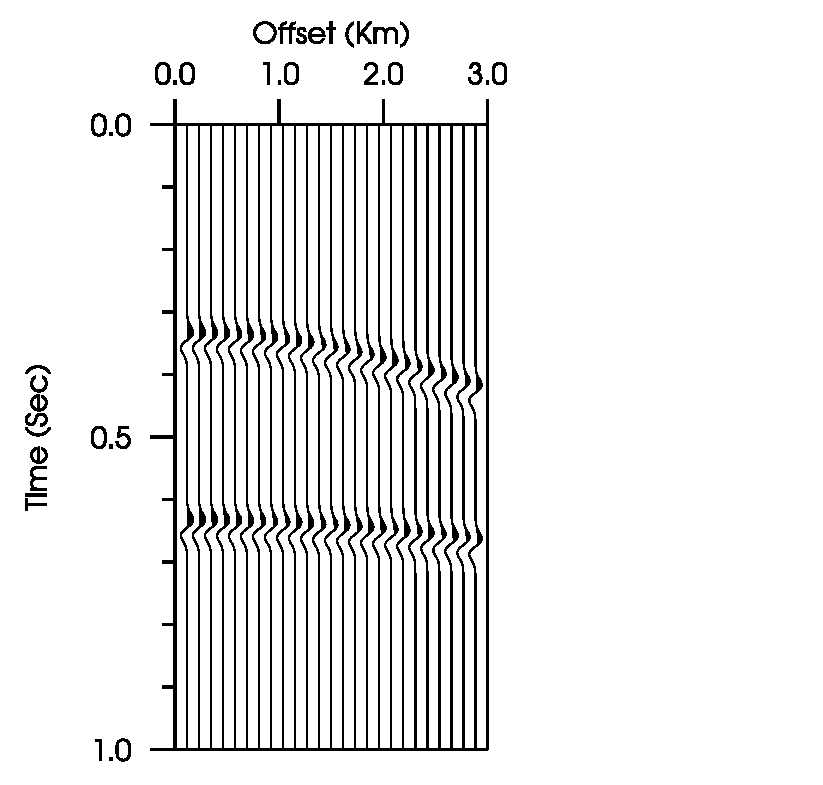
\includegraphics[width=0.75\textwidth]{Fig/fig-5-shot.pdf}
%\plot{fig-5-shot}{width=0.75\textwidth}{CMP with two events with velocity equal to 2000 m/s and 2500 m/s.}
\caption{CMP with two events with velocity equal to 2000 m/s and 2500 m/s.}
\label{fig-5-shot}
\end{figure}
\end{frame}
%============================================================
\begin{frame}
%============================================================
\begin{figure}
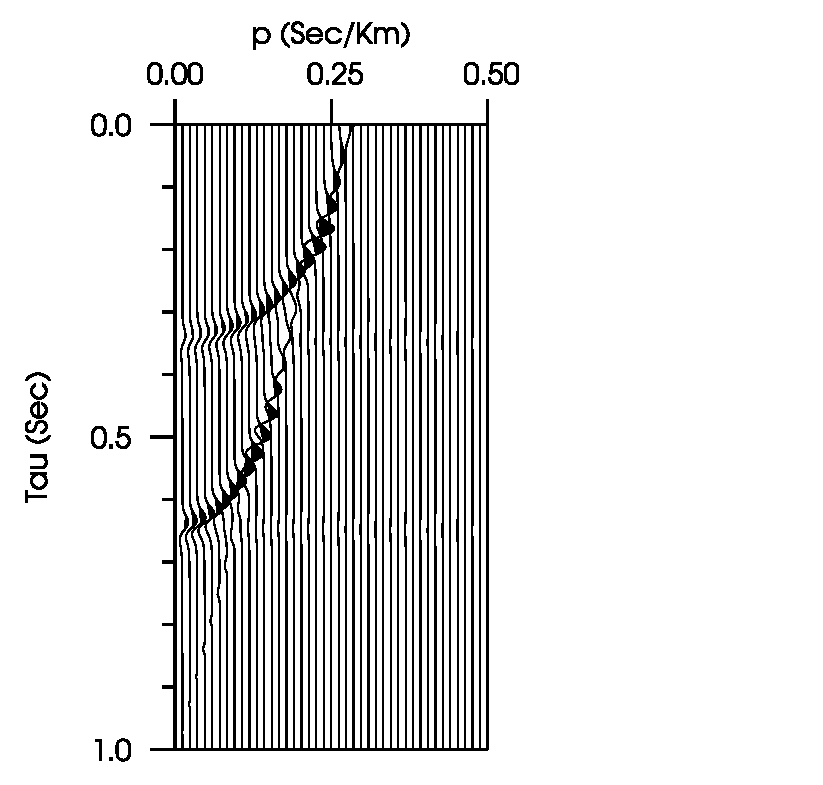
\includegraphics[width=0.75\textwidth]{Fig/fig-5-taup.pdf}
%\plot{fig-5-taup}{width=0.75\textwidth}
\caption{$\tau-p$ transform of the CMP-gather shown in figure \protect{\ref{fig-5-shot}}}
\end{figure}
\end{frame}
%
%
%============================================================
\begin{frame}{Radon Multiple removal}
%============================================================
%
\begin{itemize}
  \item Raypaths with multiple reflections
  \item Multiples are unwanted
  \item Multiples are usually removed
\end{itemize}
%============================================================
\end{frame}
%
\begin{frame}{Principle of Radon demultiple}
Traveltime-distance curve for a primary
reflection from the bottom of a layer with constant velocity
%
\begin{eqnarray}
    t_p=\sqrt{\tau^2_0 + \frac{4h^2}{c^2}},
\end{eqnarray}
%
and the first multiple reflection from the same reflector
%
\begin{eqnarray}
    t_m=\sqrt{{(2\tau_0)}^2 + \frac{ 4{(2h)}^2}{c^2}}.
\end{eqnarray}
%
\end{frame}
%
%============================================================
\begin{frame}{Principle of Radon demultiple}
%============================================================
Consider also a primary reflection arriving  from some deeper
reflector at the same time 
%
\begin{eqnarray}
    t_p=\sqrt{{(2\tau_0)}^2 + \frac{ 4{(2h)}^2}{c_{rms}^2}}.
\end{eqnarray}
%
Although arriving at the same time as the multiple reflection, the curvature of
this event is different, because the velocity is $c_{rms} > c$.
\end{frame}
\begin{frame}{Principle of Radon demultiple}
%
\begin{figure}
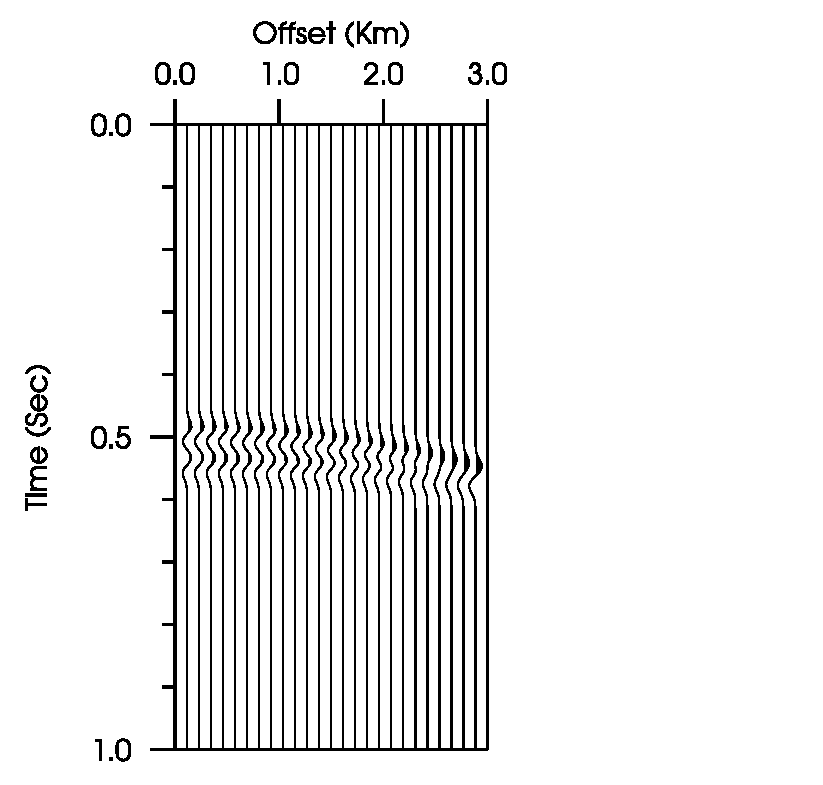
\includegraphics[width=0.6\textwidth]{Fig/fig-6-cdp.pdf}
%\plot{fig-6-cdp}{width=0.6\textwidth}
\caption{Cmp with primary reflection and multiple reflection interfering.}
\label{fig-6-cdp}
\end{figure}
\end{frame}
%
%============================================================
\begin{frame}{Principle of Radon demultiple}
%============================================================
%
\begin{figure}
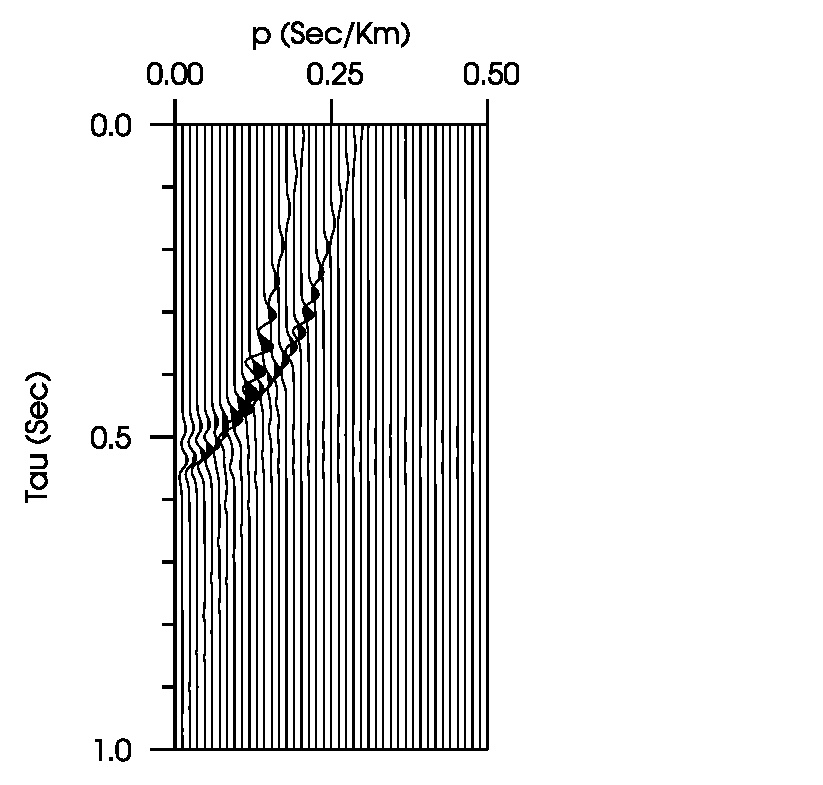
\includegraphics[width=0.6\textwidth]{Fig/fig-6-taup.pdf}
%\plot{fig-6-taup}{width=0.6\textwidth}
\caption{Cmp with primary reflection and multiple reflection from \protect{\ref{fig-6-cdp}} in the tau-p domain.
         The apparent velocity for the multiple reflection is lower than the primary reflection, 
         making separation of the two events possible.}
\end{figure}
%
\end{frame}
%
%============================================================
\begin{frame}{Principle of Radon demultiple}
%============================================================
\begin{figure}
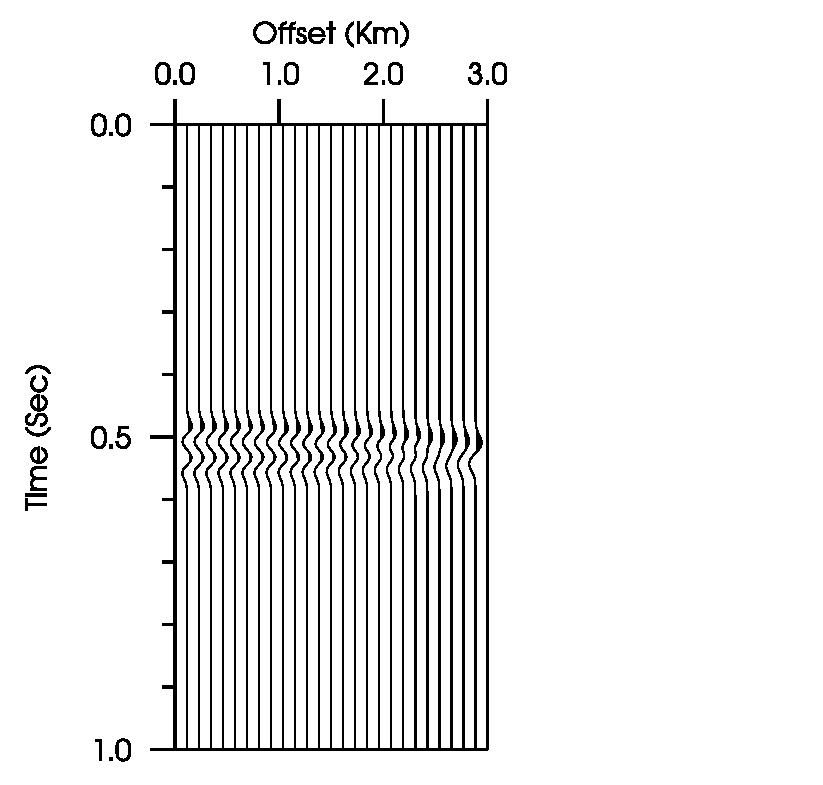
\includegraphics[width=0.6\textwidth]{Fig/fig-6-nmo.pdf}
%\plot{fig-6-nmo}{width=0.6\textwidth}
\caption{Cmp with primary reflection and multiple reflection after nmo-correction
         with a velocity higher than the multiple velocity but lower than the primary velocity.}
 \label{fig-6-nmo}
\end{figure}
\end{frame}
%============================================================
\begin{frame}{Principle of Radon demultiple}
%============================================================
\begin{figure}
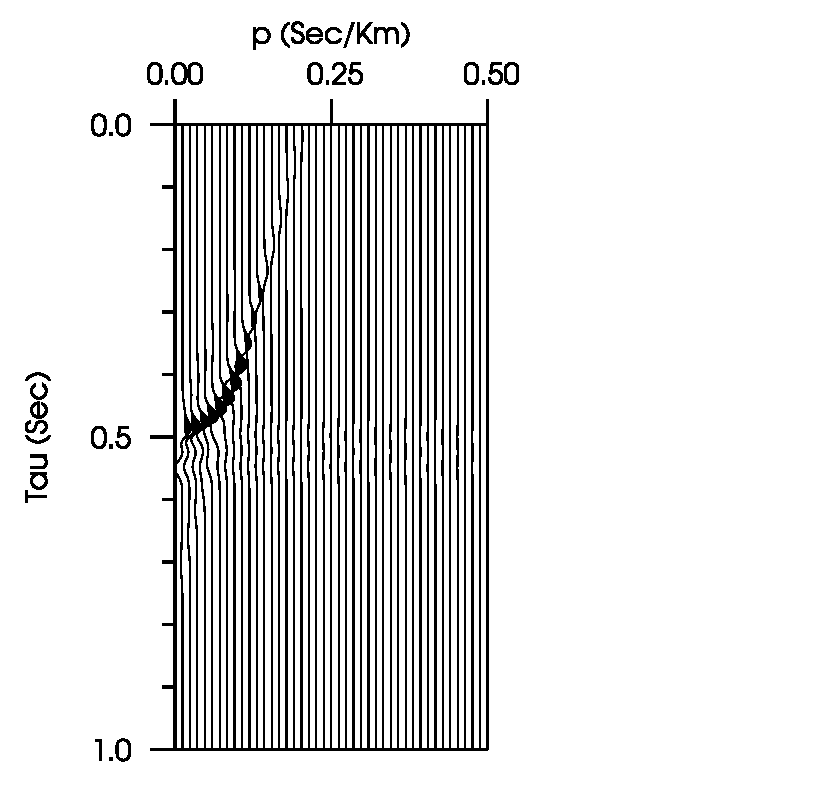
\includegraphics[width=0.6\textwidth]{Fig/fig-6-taup-nmo.pdf}
%\plot{fig-6-taup-nmo}{width=0.6\textwidth}
\caption{Cmp with primary reflection and multiple reflection  from figure \protect{\ref{fig-6-nmo}}
         after a $tau-p$-p transform. Only the multiple reflection is now visible, the primary
         appears for small negative p-values (not plotted)}.
\end{figure}
\end{frame}
%============================================================
\begin{frame}{Principle of Radon demultiple}
%============================================================
\begin{itemize}
  \item Straightforward mute and inverse transform is not possible
  \item Inverse radon gives too many artefacts
\end{itemize}
\end{frame}
%============================================================
\begin{frame}{Parabolic Radon}
%============================================================
%
\begin{eqnarray}
  \hat{f}(p,\tau) = \int^{+\infty}_{-\infty} dx \int^{+\infty}_{-\infty} dt \delta(t-px^2-\tau)f(x,t).
                   \label{eq:6-radon-para}
\end{eqnarray}
%

\begin{itemize}
 \item Transform maps an event in the x-t domain described by a parabola into a point
 \item Usefull for nmo-corrected data
\end{itemize}
\end{frame}
%============================================================
\begin{frame}{Parabolic Radon}
%============================================================
In general the inverse
transform can be considered to be of the general form
%
\begin{eqnarray}
  f(x,t) = \int^{+\infty}_{-\infty} dp \hat{f}(\tau=t-px^2,p),
                   \label{eq:6-para}
\end{eqnarray}
%
or in discrete form
%
\begin{eqnarray}
  f(x_k,t) = \sum_{l=0}^N \hat{f}(\tau=t- p_l x^2_k,p_l),
                   \label{eq:6-para-disc}
\end{eqnarray}
%
where $p_l=l\Delta p$ and $x_k = k\Delta x$. 
\end{frame}
%
%============================================================
\begin{frame}{Parabolic Radon}
%============================================================
We now want to perform a Fourier transform over the time variable
%
\begin{eqnarray}
  f(x_k,\omega) = \frac{1}{2\pi}\int^{+\infty}_{-\infty}dt \sum_{l=0}^N \hat{f}(\tau=t- p_l x^2_k,p_l)\exp(-i\omega t),
\end{eqnarray}
which becomes after substitution of variable $u=t-p_l x^2_l$
%
%
\begin{eqnarray}
  f(x_k,\omega) = \frac{1}{2\pi}\int^{+\infty}_{-\infty}du \sum_{l=0}^N \hat{f}(\tau=u,p_l)\exp[-i\omega (u+p_l x_k^2)].
\end{eqnarray}
%
The last equation is then
%
\begin{eqnarray}
  f(x_k,\omega) = \sum_{l=0}^N \hat{F}(\omega, p_l)\exp[-i\omega p_l x^2_k].
                   \label{eq:6-para-inv}
\end{eqnarray}
%
\end{frame}
%============================================================
\begin{frame}{Parabolic radon}
%============================================================
To compute the forward transform
we consider the $\hat{F}(\omega,p_l)$ as unknowns, and solve the linear system of
equations given in \eqref{eq:6-para-inv}. 
This can easily be done by writing equation \eqref{eq:6-para-inv} as a matrix equation
and using the least-squares method.
%
\begin{eqnarray}
  \mathbf{f}(\omega) = \mathbf{L}\hat{\mathbf{F}}(\omega)
                   \label{eq:6-para-inv2}
\end{eqnarray}
%
where $\mathbf{f}$ and $hat{\mathbf{F}}$ are vectors with elements $f_k=f(x_k,\omega)$ 
and $\hat{F}_k=\hat{F}(x_k)$. 
The matrix $\mathbf{L}$ have elements $L_{lk}=\exp[-i\omega p_l x^2_k$.
\end{frame}
%============================================================
\begin{frame}{Parabolic radon}
%============================================================
After muting of $\hat{\mathbf{F}}$ to remove multiples we solve the equation
\begin{eqnarray}
  \hat{\mathbf{F}}(\omega) = \mathbf{L}^{-1}\mathbf{f}(\omega)
                   \label{eq:6-para-inv3}
\end{eqnarray}
with respect to $\mathbf{f}$ to compute the inverse transform.
\end{frame}
%============================================================
\begin{frame}{Parabolic Radon}
%============================================================
%
\begin{figure}
%\plot{fig-6-data}{width=0.6\textwidth}
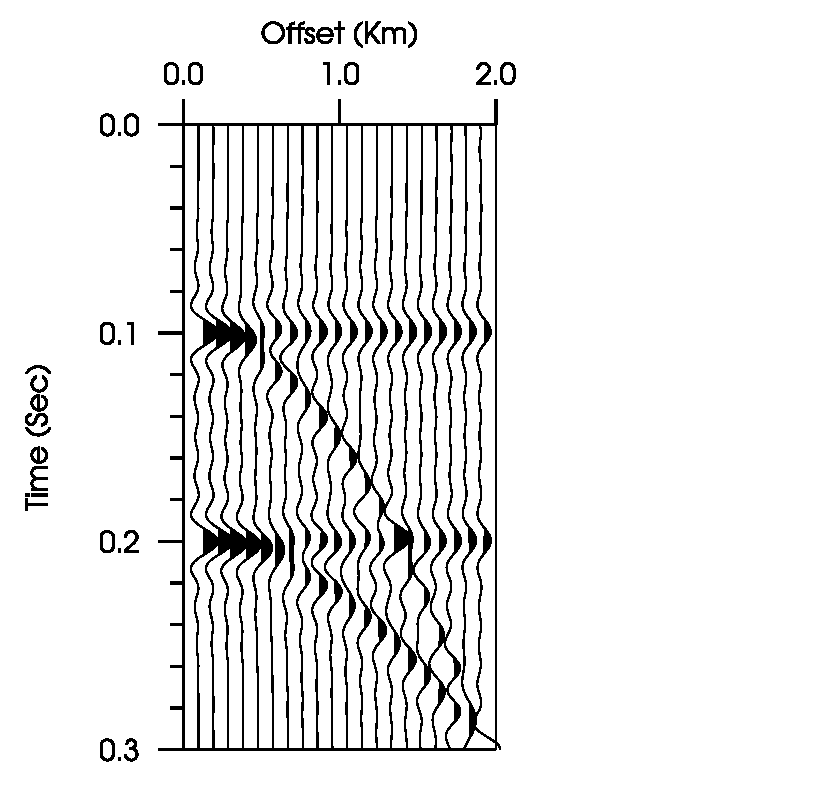
\includegraphics[width=0.6\textwidth]{Fig/fig-6-data.pdf} 
\caption{Input data with primary and multiple reflections. A normal moveout correction
         has been applied.} 
\label{fig-6-data}
\end{figure}
\end{frame}
%
%============================================================
\begin{frame}{Parabolic Radon}
%============================================================
\begin{figure}
%\plot{fig-6-radon}{width=0.6\textwidth}
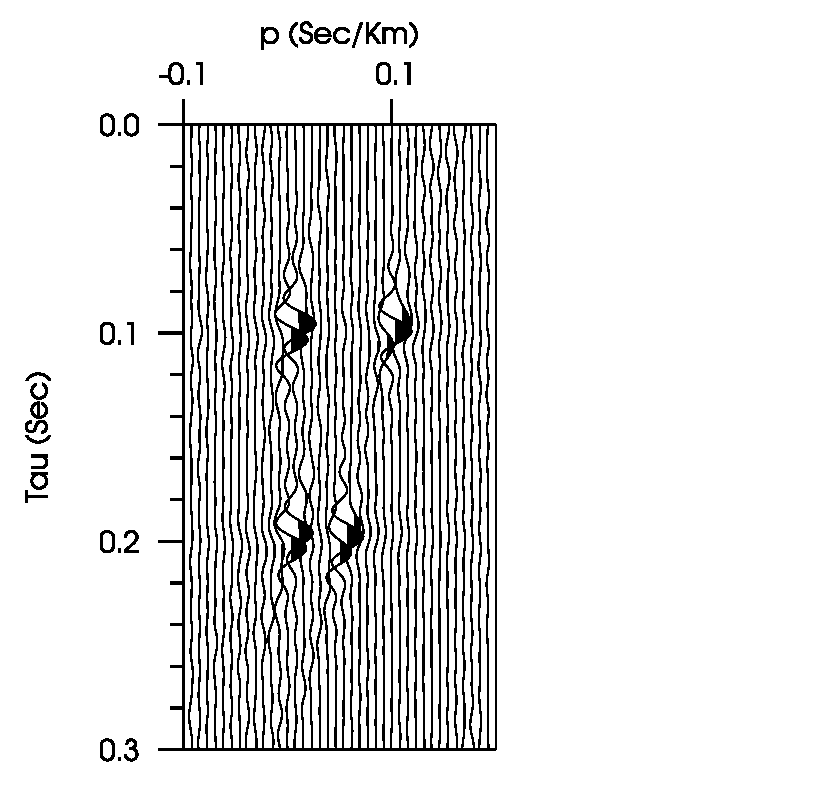
\includegraphics[width=0.6\textwidth]{Fig/fig-6-radon.pdf} 
\caption{The parabolic radon transform of the data shown in figure \protect{\ref{fig-6-data}}.}
\end{figure}
\end{frame}
%============================================================
\begin{frame}{Parabolic Radon}
%============================================================
\begin{figure}
%\plot{fig-6-prim}{width=0.6\textwidth}
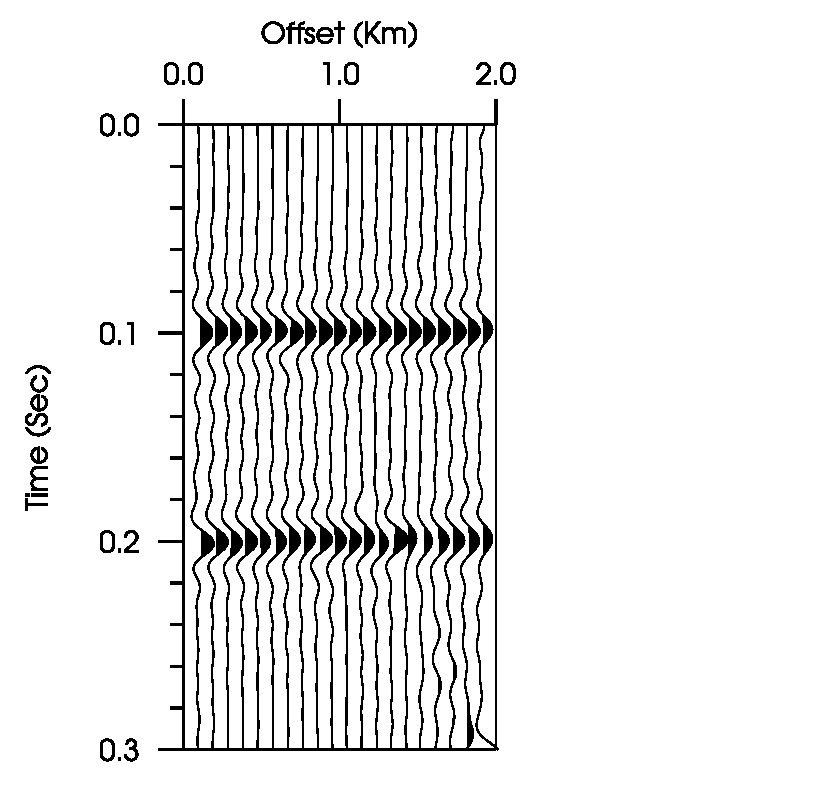
\includegraphics[width=0.6\textwidth]{Fig/fig-6-prim.pdf} 
\caption{Primary reflections estimated from the input data in figure \protect{\ref{fig-6-data}}
         using the parabolic radon transform.}
\end{figure}
\end{frame}
%
\end{document}
